\documentclass{article}
\usepackage{tikz}
\usetikzlibrary{matrix, positioning, calc}

\begin{document}

\begin{figure}[h]
    \centering
    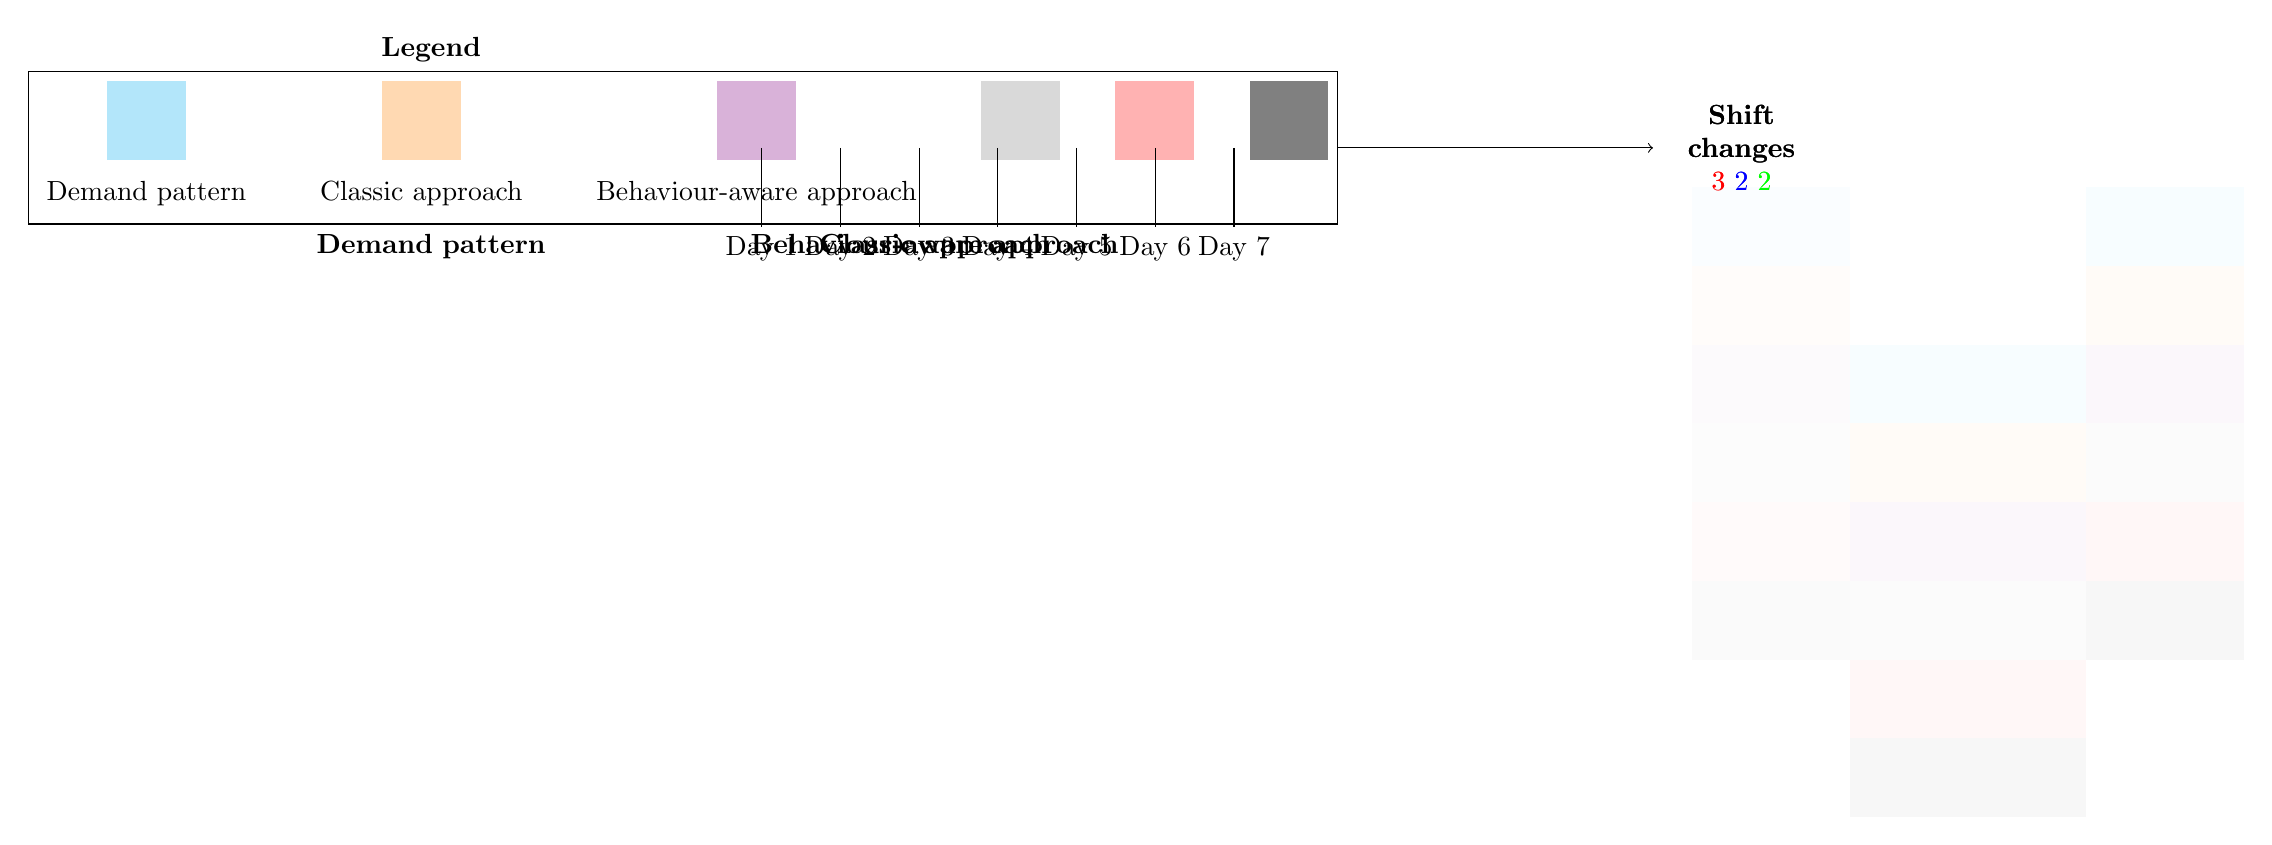
\begin{tikzpicture}[node distance=0pt, auto]
        % Legend
        \matrix (legend) [matrix of nodes, row sep=1ex, column sep=2em, draw] {
            \node[fill=cyan!30, minimum size=1cm, anchor=center] {}; & \node[fill=orange!30, minimum size=1cm, anchor=center] {}; & \node[fill=violet!30, minimum size=1cm, anchor=center] {}; & \node[fill=gray!30, minimum size=1cm, anchor=center] {}; & \node[fill=red!30, minimum size=1cm, anchor=center] {}; & \node[fill=black!50, minimum size=1cm, anchor=center] {}; \\
            Demand pattern & Classic approach & Behaviour-aware approach & & & \\
        };
        \node[above=of legend.north west, anchor=south west, text width=10cm, align=center] {\textbf{Legend}};
        \node[below=of legend.south west, anchor=north west, text width=10cm, align=center] {\textbf{Demand pattern}};
        \node[below=of legend.south east, anchor=north east, text width=10cm, align=center] {\textbf{Classic approach}};
        \node[below=of legend.south east, anchor=north east, text width=10cm, align=center] {\textbf{Behaviour-aware approach}};

        % Timeline
        \draw[->] (legend.east) -- ++(4,0) coordinate (timeline);
        \foreach \x in {1,...,7} {
            \draw (\x*1, 0) -- ++(0, -1) node[below] {Day \x};
        }

        % Classic approach
        \foreach \x/\y in {1/1, 2/1, 3/3, 4/3, 5/3, 6/1, 7/1} {
            \pgfmathtruncatemacro{\mycolor}{\x==1 ? 1 : \x==2 ? 2 : 3}
            \pgfmathtruncatemacro{\myshift}{\x==1 ? 3 : \x==2 ? 2 : 2}
            \node[fill=cyan!\mycolor, minimum size=1cm, anchor=center] at ($(timeline)+(\x,-\y)$) {};
            \node[fill=orange!\mycolor, minimum size=1cm, anchor=center] at ($(timeline)+(\x,-\y-1)$) {};
            \node[fill=violet!\mycolor, minimum size=1cm, anchor=center] at ($(timeline)+(\x,-\y-2)$) {};
            \node[fill=gray!\mycolor, minimum size=1cm, anchor=center] at ($(timeline)+(\x,-\y-3)$) {};
            \node[fill=red!\mycolor, minimum size=1cm, anchor=center] at ($(timeline)+(\x,-\y-4)$) {};
            \node[fill=black!\mycolor, minimum size=1cm, anchor=center] at ($(timeline)+(\x,-\y-5)$) {};
        }
        \node[right=of timeline, text width=2cm, align=center] {\textbf{Shift changes} \\ \textcolor{red}{3} \textcolor{blue}{2} \textcolor{green}{2}};

        % Behaviour-aware approach
        \foreach \x/\y in {1/1, 2/1, 3/3, 4/3, 5/3, 6/1, 7/1} {
            \pgfmathtruncatemacro{\mycolor}{\x==1 ? 1 : \x==2 ? 2 : 3}
            \pgfmathtruncatemacro{\myshift}{\x==1 ? 3 : \x==2 ? 2 : 2}
            \node[fill=cyan!\mycolor, minimum size=1cm, anchor=center] at ($(timeline)+(\x,-\y)$) {};
            \node[fill=orange!\mycolor, minimum size=1cm, anchor=center] at ($(timeline)+(\x,-\y-1)$) {};
            \node[fill=violet!\mycolor, minimum size=1cm, anchor=center] at ($(timeline)+(\x,-\y-2)$) {};
            \node[fill=gray!\mycolor, minimum size=1cm, anchor=center] at ($(timeline)+(\x,-\y-3)$) {};
            \node[fill=red!\mycolor, minimum size=1cm, anchor=center] at ($(timeline)+(\x,-\y-4)$) {};
            \node[fill=black!\mycolor, minimum size=1cm, anchor=center] at ($(timeline)+(\x,-\y-5)$) {};
        }
        \node[right=of timeline, text width=2cm, align=center] {\textbf{Shift changes} \\ \textcolor{red}{3} \textcolor{blue}{2} \textcolor{green}{2}};
    \end{tikzpicture}
\end{figure}

\end{document}